\documentclass{article}

\newif\ifanswers
\answerstrue

\usepackage{fancyhdr} % Required for custom headers
\usepackage{lastpage} % Required to determine the last page for the footer
\usepackage{extramarks} % Required for headers and footers
\usepackage[usenames,dvipsnames]{color} % Required for custom colors
\usepackage{graphicx} % Required to insert images
\usepackage{listings} % Required for insertion of code
\usepackage{courier} % Required for the courier font
\usepackage{lipsum} % Used for inserting dummy 'Lorem ipsum' text into the template
\usepackage{enumerate}
\usepackage{booktabs}
\usepackage{amsmath, amsthm, amssymb}
\usepackage{caption}
\usepackage{subcaption}
\captionsetup[table]{skip=4pt}
\usepackage{framed}
\usepackage{bm}
\usepackage{float}
\setcounter{section}{-1}
\usepackage{style}
\usepackage{xcolor}
\graphicspath{{img/}} % set of paths to search for images
\usepackage{amsmath}
\usepackage{amsfonts}
\usepackage{amssymb}
\usepackage[hidelinks]{hyperref}



\newenvironment{myitemize}
{ \begin{itemize}
    \setlength{\itemsep}{0pt}
    \setlength{\parskip}{0pt}
    \setlength{\parsep}{0pt}     }
  { \end{itemize}                  } 

\usepackage[backend=bibtex]{biblatex}                                               
\addbibresource{papers.bib}

\usepackage{tikz}
\usetikzlibrary{positioning,patterns,fit}

\newcommand{\ifans}[1]{\ifanswers \color{red} \textbf{Solution: } #1 \color{black} \else {} \fi}

% Margins
\topmargin=-0.45in
\evensidemargin=0in
\oddsidemargin=0in
\textwidth=6.5in
\textheight=9.0in
\headsep=0.25in

\linespread{1.1} % Line spacing

% Set up the header and footer
\pagestyle{fancy}
\rhead{\hmwkAuthorName} % Top left header
\lhead{\hmwkClass: \hmwkTitle} % Top center head
\lfoot{\lastxmark} % Bottom left footer
\cfoot{} % Bottom center footer
\rfoot{Page\ \thepage\ of\ \protect\pageref{LastPage}} % Bottom right footer
\renewcommand\headrulewidth{0.4pt} % Size of the header rule
\renewcommand\footrulewidth{0.4pt} % Size of the footer rule

\setlength\parindent{0pt} % Removes all indentation from paragraphs

%----------------------------------------------------------------------------------------
% CODE INCLUSION CONFIGURATION
%----------------------------------------------------------------------------------------

\definecolor{MyDarkGreen}{rgb}{0.0,0.4,0.0} % This is the color used for comments
\lstloadlanguages{Python} % Load Perl syntax for listings, for a list of other languages supported see: ftp://ftp.tex.ac.uk/tex-archive/macros/latex/contrib/listings/listings.pdf
\lstset{language=Python, % Use Perl in this example
        frame=single, % Single frame around code
        basicstyle=\footnotesize\ttfamily, % Use small true type font
        keywordstyle=[1]\color{Blue}\bf, % Perl functions bold and blue
        keywordstyle=[2]\color{Purple}, % Perl function arguments purple
        keywordstyle=[3]\color{Blue}\underbar, % Custom functions underlined and blue
        identifierstyle=, % Nothing special about identifiers
        commentstyle=\usefont{T1}{pcr}{m}{sl}\color{MyDarkGreen}\small, % Comments small dark green courier font
        stringstyle=\color{Purple}, % Strings are purple
        showstringspaces=false, % Don't put marks in string spaces
        tabsize=5, % 5 spaces per tab
        %
        % Put standard Perl functions not included in the default language here
        morekeywords={rand},
        %
        % Put Perl function parameters here
        morekeywords=[2]{on, off, interp},
        %
        % Put user defined functions here
        morekeywords=[3]{test},
        %
        morecomment=[l][\color{Blue}]{...}, % Line continuation (...) like blue comment
        numbers=left, % Line numbers on left
        firstnumber=1, % Line numbers start with line 1
        numberstyle=\tiny\color{Blue}, % Line numbers are blue and small
        stepnumber=5 % Line numbers go in steps of 5
}

% Creates a new command to include a perl script, the first parameter is the filename of the script (without .pl), the second parameter is the caption
\newcommand{\perlscript}[2]{
\begin{itemize}
\item[]\lstinputlisting[caption=#2,label=#1]{#1.pl}
\end{itemize}
}

%----------------------------------------------------------------------------------------
% NAME AND CLASS SECTION
%----------------------------------------------------------------------------------------

\newcommand{\hmwkTitle}{Assignment \#2} % Assignment title
\newcommand{\hmwkClass}{CS\ 234 Winter 2021} % Course/class
\newcommand{\hmwkAuthorName}{} % Your name

%----------------------------------------------------------------------------------------
% TITLE PAGE
%----------------------------------------------------------------------------------------

\title{
\vspace{-1in}
\textmd{\textbf{\hmwkClass:\ \hmwkTitle}}}
\author{}    
\date{} % Insert date here if you want it to appear below your name

\begin{document}

\maketitle
\vspace{-.5in}
\begin{framed}
{\bf Due date: \\
Part 1 (0-4): February 5, 2021 at 6 PM (18:00) PST\\
Part 2 (5-6): February 12, 2021 at 6 PM (18:00) PST}
\\[1em]
These questions require thought, but do not require long answers. Please be as concise as possible.
\\[1em]
We encourage students to discuss in groups for assignments. We ask
that you abide by the university Honor Code and that of the Computer Science department. If you have discussed the problems with others,
please include a statement saying who you discussed problems with. Failure to follow these instructions
will be reported to the Office of Community Standards. We reserve the right to run a fraud-detection software on your code. Please refer to \href{http://web.stanford.edu/class/cs234/index.html}{website}, Academic Collaboration and Misconduct section for details about collaboration policy.


Please review any additional instructions posted on the assignment page. When you are ready to submit, please
follow the instructions on the course website. \textbf{Make sure you test your code using the
provided commands and do not edit outside of the marked areas.}
\\[1em]
You'll need to download the starter code and fill the appropriate functions following the instructions from the handout and the code's documentation. Training DeepMind's network on \texttt{Pong} takes roughly \textbf{12 hours on GPU}, so \textbf{please start early}! (Only a completed run will recieve full credit) We will give you access to an Azure GPU cluster. You'll find the setup instructions on the course assignment page.
\end{framed}
\section*{Introduction}

In this assignment we will implement deep Q-learning, following DeepMind's paper (\cite{mnih2015human} and \cite{mnih-atari-2013}) that learns to play Atari games from raw pixels. The purpose is to demonstrate the effectiveness of deep neural networks as well as some of the techniques used in practice to stabilize training and achieve better performance. In the process, you'll become familiar with PyTorch. We will train our networks on the \texttt{Pong} environment from Gymnasium (former OpenAI Gym), but the code can easily be applied to any other environment. \\

In Pong, one player scores if the ball passes by the other player. An episode is over when one of the players reaches $21$ points. Thus, the total return of an episode is between $-21$ (lost every point) and $+21$ (won every point). Our agent plays against a decent hard-coded AI player. Average human performance is $-3$ (reported in \cite{mnih-atari-2013}). In this assignment, you will train an AI agent with super-human performance, reaching at least $+10$ (hopefully more!).


\newpage

\section{Distributions induced by a policy (13 pts)}
In this problem, we'll work with an infinite-horizon MDP $\mathcal{M} = \langle \mathcal{S}, \mathcal{A}, \mathcal{R}, \mathcal{T}, \gamma \rangle$ and consider stochastic policies of the form $\pi: \mathcal{S} \rightarrow \Delta(\mathcal{A})$\footnote{For a finite set $\mathcal{X}$, $\Delta(\mathcal{X})$ refers to the set of categorical distributions with support on $\mathcal{X}$ or, equivalently, the $\Delta^{|\mathcal{X}|-1}$ probability simplex.}. Additionally, we'll assume that $\mathcal{M}$ has a single, fixed starting state $s_0 \in \mathcal{S}$ for simplicity.
\begin{enumerate}[(a)]
	\item (\textbf{written}, 3 pts) Consider a fixed stochastic policy and imagine running several rollouts of this policy within the environment. Naturally, depending on the stochasticity of the MDP $\mathcal{M}$ and the policy itself, some trajectories are more likely than others. Write down an expression for $\rho^\pi(\tau)$, the likelihood of sampling a trajectory $\tau = (s_0,a_0,s_1,a_1,\ldots)$ by running $\pi$ in $\mathcal{M}$. To put this distribution in context, recall that $V^\pi(s_0) = \mathbb{E}_{\tau \sim \rho^\pi}\left[\sum\limits_{t=0}^\infty \gamma^t \mathcal{R}(s_t,a_t) \,|\, s_0\right].$
	
	\ifans{
	}
	
	\item (\textbf{written}, 5 pts) Just as $\rho^\pi$ captures the distribution over trajectories induced by $\pi$, we can also examine the distribution over states induced by $\pi$. In particular, define the \textit{discounted, stationary state distribution} of a policy $\pi$ as $$d^\pi(s) = (1-\gamma) \sum\limits_{t=0}^\infty \gamma^t p(s_t = s),$$ where $p(s_t = s)$ denotes the probability of being in state $s$ at timestep $t$ while following policy $\pi$; your answer to the previous part should help you reason about how you might compute this value. Consider an arbitrary function $f: \mathcal{S} \times \mathcal{A} \rightarrow \mathbb{R}$. Prove the following identity: $$\mathbb{E}_{\tau \sim \rho^\pi}\left[\sum\limits_{t=0}^\infty \gamma^t f(s_t,a_t)\right] = \frac{1}{(1-\gamma)} \mathbb{E}_{s \sim d^\pi}\left[\mathbb{E}_{a \sim \pi(s)}\left[f(s,a)\right]\right] .$$ 
	\emph{Hint: You may find it helpful to first consider how things work out for $f(s,a) = 1, \forall (s,a) \in \mathcal{S} \times \mathcal{A}$.}\\
	\emph{Hint: What is $p(s_t=s)$?}
	
	\ifans{
	}
	
	\item (\textbf{written}, 5 pts) For any policy $\pi$, we define the following function $$A^\pi(s,a) = Q^\pi(s,a) - V^\pi(s).$$ Prove the following statement holds for all policies $\pi,\pi'$: $$V^\pi(s_0) - V^{\pi'}(s_0) = \frac{1}{(1-\gamma)} \mathbb{E}_{s \sim d^\pi}\left[\mathbb{E}_{a \sim \pi(s)}\left[A^{\pi'}(s,a)\right]\right].$$
	
	\ifans{
	}
\end{enumerate}

\section{Test Environment (6 pts)}
Before running our code on Pong, it is crucial to test our code on a test environment. In this problem, you will reason about optimality in the provided test environment by hand; later, to sanity-check your code, you will verify that your implementation is able to achieve this optimality. You should be able to run your models on CPU in no more than a few minutes on the following environment:

\begin{itemize}
	\item $ 4 $ states: $ 0, 1, 2, 3 $
	\item $ 5 $ actions: $ 0, 1, 2, 3, 4 $. Action $ 0 \leq i \leq 3 $ goes to state $ i $, while action $ 4 $ makes the agent stay in the same state.
	\item Rewards: Going to state $ i $ from states 0, 1, and 3 gives a reward $R(i) $, where $R(0) = 0.2, R(1) = -0.1, R(2) = 0.0, R(3) = -0.3 $. If we start in state $ 2 $, then the rewards defind above are multiplied by $ - 10 $.  See Table~\ref{tab:TestEnv} for the full transition and reward structure. 
	\item One episode lasts 5 time steps (for a total of 5 actions) and always starts in state $ 0 $ (no rewards at the initial state).        
\end{itemize}

\begin{center}
	\begin{tabular}{ | l | l | l | l |}  
		\hline
		State ($s$) & Action ($a$) & Next State ($s'$) & Reward ($R$) \\ \hline
		0 & 0 & 0 & 0.2    \\ \hline
		0 & 1 & 1 & -0.1   \\ \hline
		0 & 2 & 2 & 0.0 \\ \hline
		0 & 3 & 3 & -0.3 \\ \hline
		0 & 4 & 0 & 0.2 \\ \hline
		1 & 0 & 0 & 0.2    \\ \hline
		1 & 1 & 1 & -0.1   \\ \hline
		1 & 2 & 2 & 0.0 \\ \hline
		1 & 3 & 3 & -0.3 \\ \hline
		1 & 4 & 1 & -0.1 \\ \hline
		2 & 0 & 0 & -2.0    \\ \hline
		2 & 1 & 1 & 1.0   \\ \hline
		2 & 2 & 2 & 0.0 \\ \hline
		2 & 3 & 3 & 3.0 \\ \hline
		2 & 4 & 2 & 0.0 \\ \hline
		3 & 0 & 0 & 0.2    \\ \hline
		3 & 1 & 1 & -0.1   \\ \hline
		3 & 2 & 2 & 0.0 \\ \hline
		3 & 3 & 3 & -0.3 \\ \hline
		3 & 4 & 3 & -0.3 \\ \hline    
	\end{tabular}
	\captionof{table}{Transition table for the Test Environment} \label{tab:TestEnv} 
\end{center}

An example of a trajectory (or episode) in the test environment is shown in Figure \ref{fig:test_env}, and the trajectory can be represented in terms of $s_t, a_t, R_t$ as: 
$s_0 = 0, a_0=1, R_0 = -0.1, s_1=1, a_1=2, R_1 = 0.0, s_2=2, a_2=4, R_2 = 0.0, s_3=2, a_3=3, R_3  = 3.0, s_4=3, a_4=0, R_4 = 0.2, s_5=0 $.

\begin{figure}[H]
  \centering
  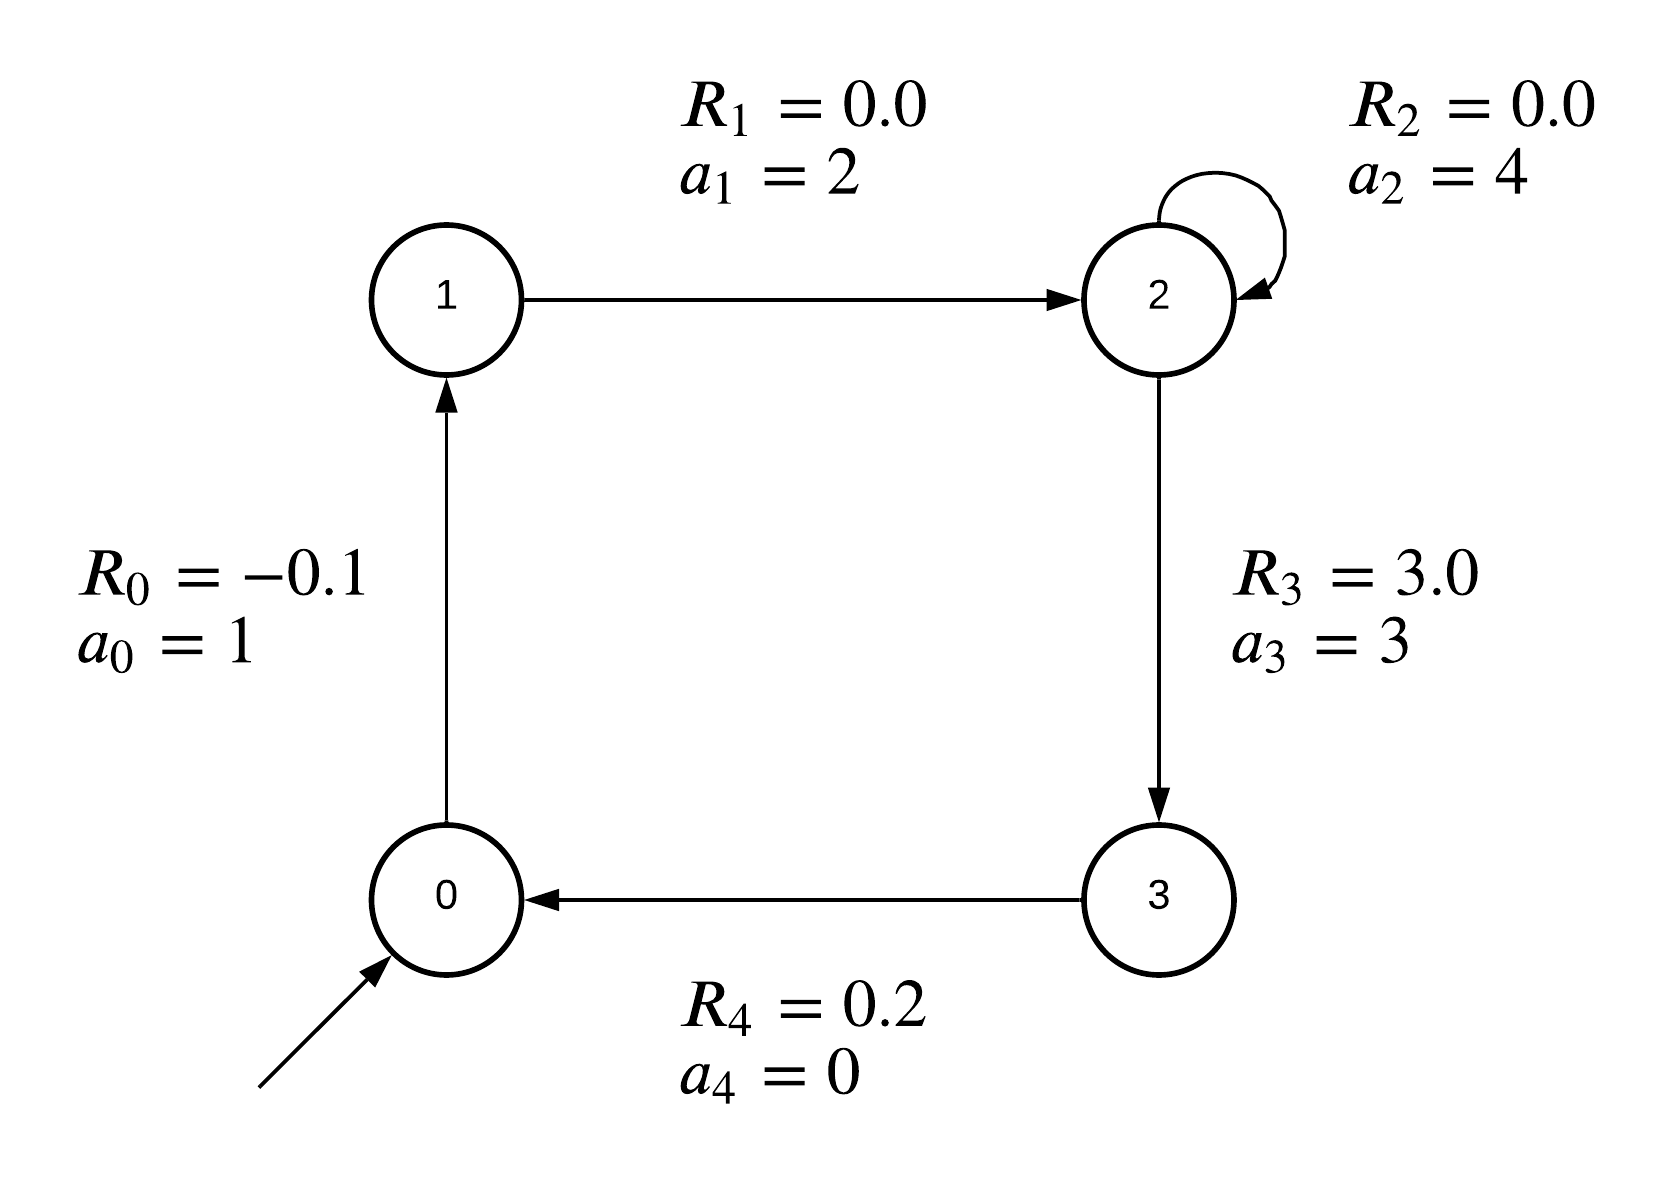
\includegraphics[width=.45\linewidth]{test_env}
  \caption{Example of a trajectory in the Test Environment}
  \label{fig:test_env}
\end{figure}

\begin{enumerate}[(a)]
\item (\textbf{written} 6 pts) What is the maximum sum of rewards that can be achieved in a single trajectory in the test environment, assuming $\gamma = 1$? Show first that this value is attainable in a single trajectory, and then briefly argue why no other trajectory can achieve greater cumulative reward.
\end{enumerate}

\ifans{
}


\section{Tabular Q-Learning (8 pts)}\label{tabular-q-learn}
If the state and action spaces are sufficiently small, we can simply maintain a table containing the value of $Q(s,a)$, an estimate of $Q^*(s,a)$, for every $(s,a)$ pair.
In this \emph{tabular setting}, given an experience sample $(s, a, r, s')$, the update rule is
\begin{equation}
Q(s,a) \leftarrow Q(s,a) + \alpha\left(r + \gamma \max_{a' \in \mathcal{A}}Q(s',a') - Q(s,a)\right) \label{eqn:tabularq}
\end{equation}
where $\alpha > 0$ is the learning rate, $\gamma \in [0,1)$ the discount factor.

\paragraph{$\epsilon$-Greedy Exploration Strategy}
For exploration, we use an $\epsilon$-greedy strategy.
This means that with probability $\epsilon$, an action is chosen uniformly at random from $\mathcal{A}$, and with probability $1-\epsilon$, the greedy action (i.e., $\arg\max_{a \in \mathcal{A}} Q(s,a)$) is chosen.
\begin{enumerate}[(a)]
\item (\textbf{coding}, 3 pts) Implement the \texttt{get\_action} and \texttt{update} functions in \texttt{q2\_schedule.py}. Test your implementation by running \texttt{python q2\_schedule.py}.	
\end{enumerate}


\paragraph{Overestimation bias}
We will now examine the issue of overestimation bias in Q-learning. The crux of the problem is that, since we take a max over actions, errors which cause Q to overestimate will tend to be amplified when computing the target value, while errors which cause Q to underestimate will tend to be suppressed.

\begin{enumerate}[(b)]
\item (\textbf{written}, 5 pts) Assume for simplicity that our Q function is an unbiased estimator of $Q^*$, meaning that $\mathbb{E}[Q(s,a)] = Q^*(s,a)$ for all states $s$ and actions $a$. (Note that this expectation is over the randomness in $Q$ resulting from the stochasticity of the exploration process.)
Show that, even in this seemingly benign case, the estimator overestimates the real target in the following sense:
$$
\forall s, \quad \mathbb{E}\left[ \max_a Q(s,a) \right] \ge \max_a Q^*(s,a)
$$

\ifans{
}
\end{enumerate}


\section{Q-Learning with Function Approximation (13 points)} 
Due to the scale of Atari environments, we cannot reasonably learn and store a Q value for each state-action tuple. We will instead represent our Q values as a parametric function $Q_{\theta}(s,a)$ where $\theta \in \mathbb{R}^p$ are the parameters of the function (typically the weights and biases of a linear function or a neural network). In this \emph{approximation setting}, the update rule becomes
\begin{equation}
\theta \leftarrow \theta + \alpha\left(r+\gamma \max_{a' \in \mathcal{A}} Q_{\theta}(s', a') - Q_{\theta}(s, a)\right) \nabla_{\theta}Q_{\theta}(s, a) \label{eqn:faq}
\end{equation}
where $(s,a,r,s')$ is a transition from the MDP.\\

To improve the data efficiency and stability of the training process, DeepMind's paper \cite{mnih2015human} employed two strategies:
\begin{itemize}
	\item A \textit{replay buffer} to store transitions observed during training. When updating the $Q$ function, transitions are drawn from this replay buffer. This improves data efficiency by allowing each transition to be used in multiple updates.
	
	\item A \textit{target network} with parameters $\bar{\theta}$ to compute the target value of the next state, $\max_{a'} Q(s',a')$. The update becomes
	\begin{equation}
	\theta \leftarrow \theta + \alpha\left(r+\gamma \max_{a' \in \mathcal{A}}Q_{\bar{\theta}}\left(s', a'\right) - Q_{\theta}(s, a)\right) \nabla_{\theta} Q_{\theta}(s, a) \label{eqn:target-update}
	\end{equation}
\end{itemize}

Updates of the form \eqref{eqn:target-update} applied to transitions sampled from a replay buffer $\mathcal{D}$ can be interpreted as performing stochastic gradient descent on the following objective function: 
\begin{equation}
L_{\text{DQN}}(\theta) = \underset{(s,a,r,s') \sim \mathcal{D}}{\mathbb{E}}\left[\left(r+\gamma \max_{a' \in \mathcal{A}}Q_{\bar{\theta}}(s', a') - Q_{\theta}(s, a)\right)^2\right] \label{eqn:brm}
\end{equation}
Note that this objective is also a function of both the replay buffer $\mathcal{D}$ and the target network $Q_{\bar{\theta}}$.
The target network parameters $\bar{\theta}$ are held fixed and not updated by SGD, but periodically -- every $C$ steps -- we synchronize by copying $\bar{\theta} \leftarrow \theta$.\\

We will now examine some implementation details.
\begin{enumerate}[(a)]

\item (\textbf{written} 3 pts) DeepMind's deep Q network (DQN) takes as input the state $s$ and outputs a vector of size $|\mathcal{A}|$, the number of actions. What is one benefit of computing the $Q$ function as $Q_{\theta}(s, \cdot) \in \mathbb{R}^{|\mathcal{A}|}$, as opposed to $Q_{\theta}(s, a) \in \mathbb{R}$?

\ifans{
}

\item (\textbf{written} 5 pts) Describe the tradeoff at play in determining a good choice of $C$. In particular, why might it not work to take a very small value such as $C = 1$? Conversely, what is the consequence of taking $C$ very large? What happens if $C = \infty$?

\ifans{
}

\item (\textbf{written}, 5 pts) In supervised learning, the goal is typically to minimize a predictive model's error on data sampled from some distribution.
If we are solving a regression problem with a one-dimensional output, and we use mean-squared error to evaluate performance, the objective writes
\[
L(\theta) = \underset{(\mathbf{x},y) \sim \mathcal{D}}{\mathbb{E}}[(y - f_{\theta}(\mathbf{x}))^2]
\]
where $\mathbf{x}$ is the input, $y$ is the output to be predicted from $\mathbf{x}$, $\mathcal{D}$ is a dataset of samples from the (unknown) joint distribution of $\mathbf{x}$ and $y$, and $f_{\theta}$ is a predictive model parameterized by $\theta$.

This objective looks very similar to the DQN objective \eqref{eqn:brm}. How are these two scenarios different? (There are at least two significant differences.)

\ifans{
}
\end{enumerate}

\section{Linear Approximation (23 pts)}
\begin{enumerate}[(a)]
\item (\textbf{written}, 5 pts) 
Suppose we represent the $Q$ function as
$Q_{\theta}(s, a) = \theta^\top \delta(s,a)$, where $\theta \in \mathbb{R}^{\vert\mathcal{S}\vert \vert \mathcal{A}\vert }$ and $\delta : \mathcal{S} \times \mathcal{A} \rightarrow \mathbb{R}^{|\mathcal{S}| |\mathcal{A}|}$ with
\[
    [\delta(s,a)]_{s',a'}=\left\{
                \begin{array}{ll}
                  1 & \text{ if } s'=s, a'=a\\
                  0 & \text{otherwise}\\
                \end{array}
              \right.
  \]
  
  Compute $\nabla_{\theta} Q_{\theta}(s, a)$ and write the update rule for $\theta$.
  Argue that equations \eqref{eqn:tabularq} and \eqref{eqn:faq} from above are exactly the same when this form of linear approximation is used.
  
 \ifans{
  }

 
\item (\textbf{coding}, 15 pts) We will now implement linear approximation in PyTorch. This question will set up the pipeline for the remainder of the assignment. You'll need to implement the following functions in \texttt{q3\_linear\_torch.py} (please read through \texttt{q3\_linear\_torch.py}):
\begin{itemize}
	\item \texttt{initialize\_models}
	\item \texttt{get\_q\_values}
	\item \texttt{update\_target}
	\item \texttt{calc\_loss}
	\item \texttt{add\_optimizer}
\end{itemize}
Test your code by running \texttt{python q3\_linear\_torch.py} \textbf{locally on CPU}.  This will run linear approximation with PyTorch on the test environment from Problem 0.  Running this implementation should only take a minute.

\item (\textbf{written}, 3 pts) Do you reach the optimal achievable reward on the test environment? Attach the plot \texttt{scores.png} from the directory \texttt{results/q3\_linear} to your writeup.
 
 \ifans{
}

\end{enumerate}


\section{Implementing DeepMind's DQN (13 pts)}

\begin{enumerate}[(a)]

\item (\textbf{coding} 10pts) Implement the deep Q-network as described in \cite{mnih2015human} by implementing \texttt{initialize\_models} and \texttt{get\_q\_values} in \texttt{q4\_nature\_torch.py}. The rest of the code inherits from what you wrote for linear approximation. Test your implementation \textbf{locally on CPU} on the test environment by running \texttt{python q4\_nature\_torch.py}.  Running this implementation should only take a minute or two.

\item (\textbf{written} 3 pts) Attach the plot of scores, \texttt{scores.png}, from the directory \texttt{results/q4\_nature} to your writeup. Compare this model with linear approximation. How do the final performances compare? How about the training time? 

\ifans{
}

\end{enumerate}

\section{DQN on Atari (21 pts)}

Reminder: Please remember to kill your VM instances when you are done using them!! \\

The Atari environment from Gymnasium (former OpenAI gym) returns observations (or original frames) of size $ (210 \times 160 \times 3) $, the last dimension corresponds to the RGB channels filled with values between $ 0 $ and $ 255 $ (\texttt{uint8}). Following DeepMind's paper \cite{mnih2015human}, we will apply some preprocessing to the observations:   
\begin{myitemize}
\item Single frame encoding: To encode a single frame, we take the maximum value for each pixel color value over the frame being encoded and the previous frame. In other words, we return a pixel-wise max-pooling of the last 2 observations.     
\item Dimensionality reduction: Convert the encoded frame to grey scale, and rescale it to $(80 \times 80 \times 1)$. (See Figure \ref{fig:pong_env})     
\end{myitemize}

The above preprocessing is applied to the 4 most recent observations and these encoded frames are stacked together to produce the input (of shape $(80 \times 80 \times 4)$) to the Q-function. Also, for each time we decide on an action, we perform that action for 4 time steps. This reduces the frequency of decisions without impacting the performance too much and enables us to play 4 times as many games while training. You can refer to the \textit{Methods Section} of \cite{mnih2015human} for more details.       \\  

\begin{figure}[H]
\centering
\begin{subfigure}[b]{.5\textwidth}
  \centering
  
\includegraphics[width=.25\linewidth]{pong}
  \caption{Original input $ (210 \times 160 \times 3) $ with RGB colors}
  \label{fig:pong}
\end{subfigure}
\begin{subfigure}[b]{.5\textwidth}
  \centering
  
\includegraphics[width=.15\linewidth]{pong_grey}
  \caption{After preprocessing in grey scale of shape $ (80 \times 80 \times 1 ) $}
  \label{fig:pong_grey}
\end{subfigure}
\caption{\texttt{Pong} environment}
\label{fig:pong_env}
\end{figure}

\begin{enumerate}[(a)]
\item (\textbf{coding and written}, 5 pts). Now we're ready to train on the Atari \texttt{Pong} environment. First, launch linear approximation on pong with \texttt{python q5\_train\_atari\_linear.py} \textbf{on Azure's GPU}. This will train the model for 500,000 steps and should take approximately half an hour.  Briefly qualitatively describe how your agent's performance changes over the course of training. Do you think that training for a larger number of steps would likely yield further improvements in performance? Explain your answer.

\ifans{
}

\item (\textbf{coding and written}, 10 pts). In this question, we'll train the agent with DeepMind's architecture on the Atari \texttt{Pong} environment. Run \texttt{python q6\_train\_atari\_nature.py} \textbf{on Azure's GPU}.  This will train the model for 4 million steps. To speed up training, we have trained the model for 2 million steps. You are responsible for training it to completion, which should take \textbf{12 hours}. Attach the plot \texttt{scores.png} from the directory \texttt{results/q6\_train\_atari\_nature} to your writeup.
You should get a score of around 11-13 after 4 million total time steps.  As stated previously, the DeepMind paper claims average human performance is $ -3 $.


\ifans{
}

As the training time is roughly 12 hours, you may want to check after a few epochs that your network is making progress.  The following are some training tips:

\begin{myitemize}
\item If you terminate your terminal session, the training will stop.  In order to avoid this, you should use \texttt{screen} to run your training in the background.
\item The evaluation score printed on terminal should start at -21 and increase.
\item The max of the q values should also be increasing
\item The standard deviation of q shouldn't be too small. Otherwise it means that all states have similar q values
\item You may want to use Tensorboard to track the history of the printed metrics. You can monitor your training with Tensorboard by typing the command \texttt{tensorboard --logdir=results} and then connecting to \texttt{ip-of-you-machine:6006}.  Below are our Tensorboard graphs from one training session:
\end{myitemize}

\begin{figure}[H]
\centering
  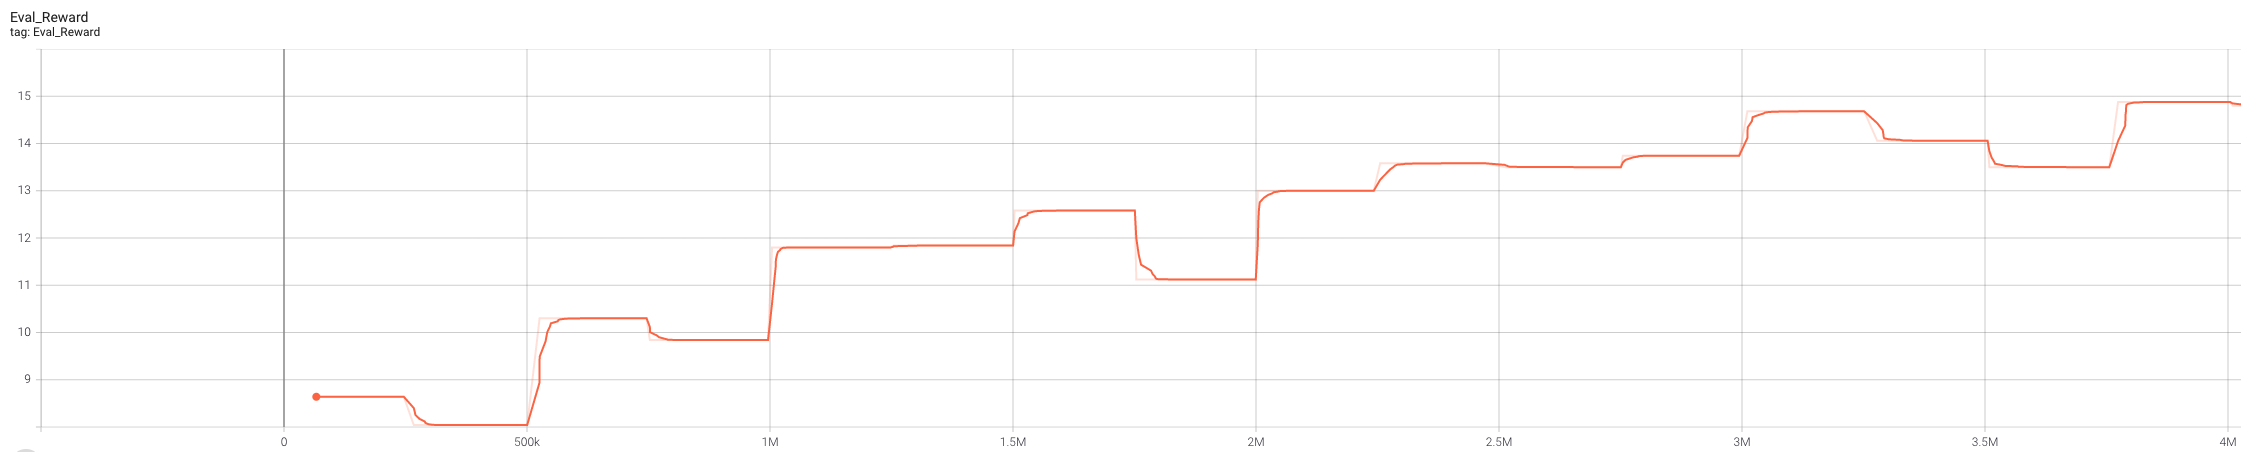
\includegraphics[width=.4\linewidth]{Eval_R.png}
  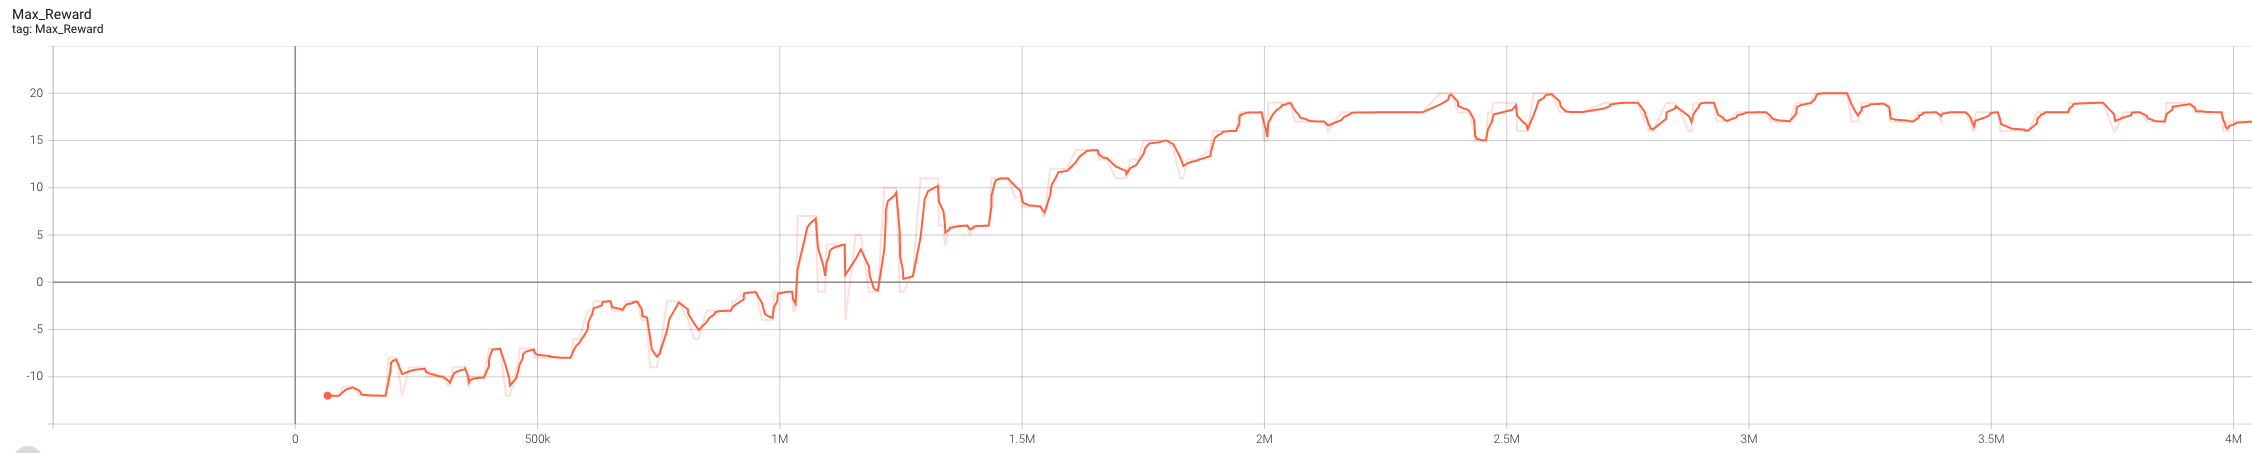
\includegraphics[width=.4\linewidth]{Max_R.png}
  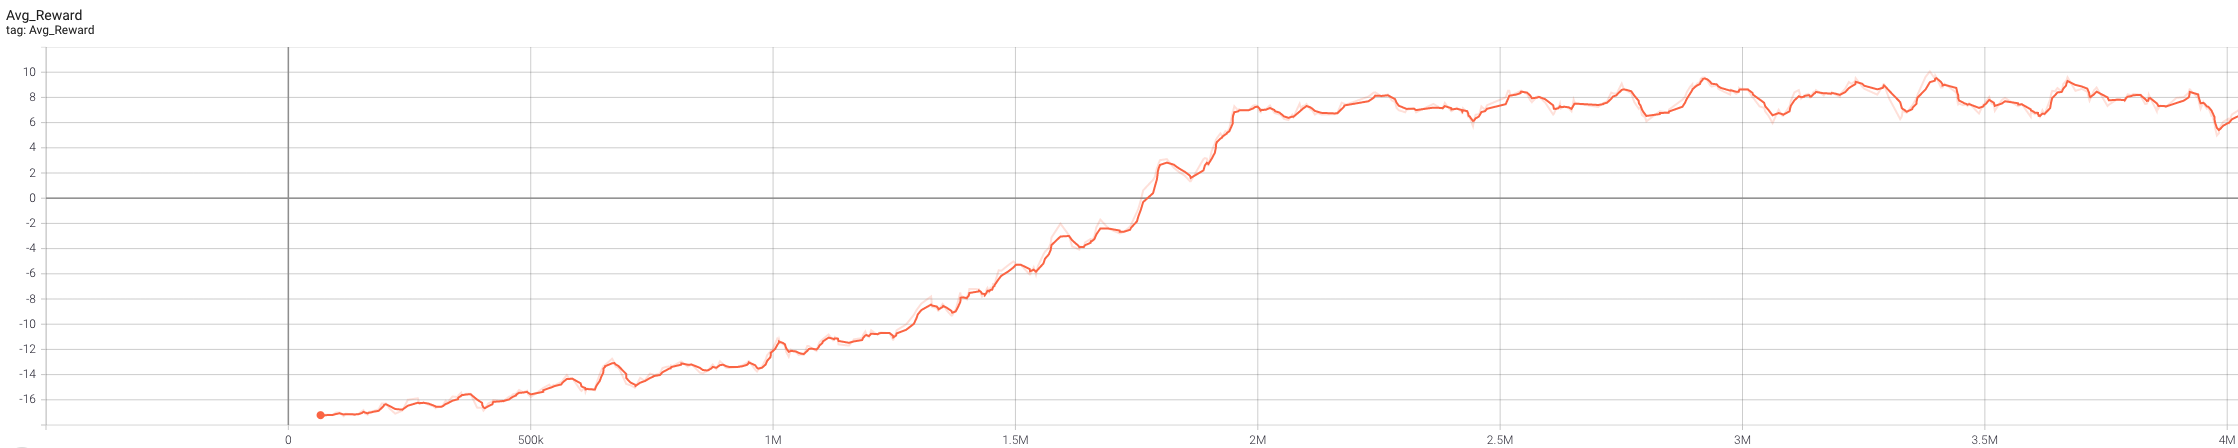
\includegraphics[width=.4\linewidth]{Avg_R.png}
  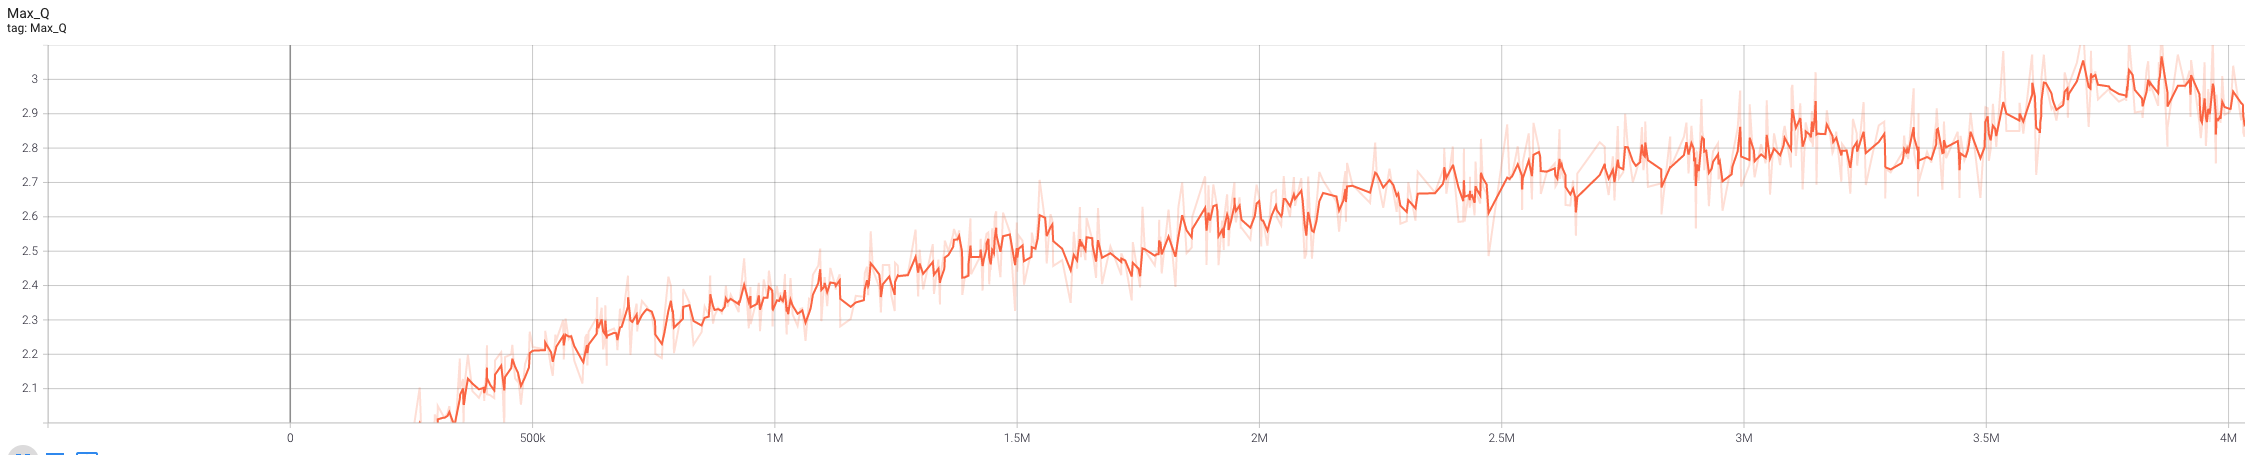
\includegraphics[width=.4\linewidth]{Max_Q.png}
\end{figure}

\item (\textbf{written}, 3 pts) In a few sentences, compare the performance of the DeepMind DQN architecture with the linear Q value approximator. How can you explain the gap in performance?

\ifans{
}

\item (\textbf{written}, 3 pts) Will the performance of DQN over time always improve monotonically? Why or why not? 

\ifans{
}

\end{enumerate}

\printbibliography

\end{document}
